\documentclass[12pt]{article}
\usepackage[margin=1in]{geometry}     
\usepackage{graphicx}
\usepackage{epstopdf}
\setlength\parindent{0pt}
\usepackage{natbib}
\usepackage{booktabs}
\bibliographystyle{plainnat}
\usepackage[format=plain,
labelfont=it,
textfont=it]{caption}

%opening
\title{Controls on Sea-Air CO$_{2}$ Flux in EBUS}
\author{Riley X. Brady}
\date{\today}


\begin{document}

\maketitle
\begin{abstract}
\noindent Working to understand what controls historical variability in Sea-Air CO$_{2}$ Flux in Eastern Boundary Upwelling Systems. I use FG\_CO2 output from the CESM Large Ensemble and correlate it to various climate indices derived from model output.
\end{abstract}

\section{California Current}

\subsection{Study Site}
For simplicity, I am using the latitudinal bounds set up by \citet{Chavez:2009}. This equates to 34N - 44N for the CCS. In terms of longitude, I want to approach it similarly to \citet{Turi:2014}. In the future, I can make this banded if needed (0-100km, 100-400km, etc.), but for now, 4 regions by 3 bands per region is a lot to work with. Instead, I am just restricting it to 800km offshore and bounded by 10 degrees of latitude for standardization.
\begin{figure}[!h]
	\centering
	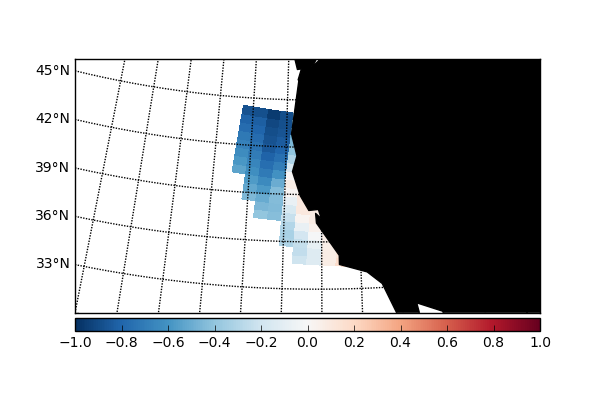
\includegraphics[width=19pc]{../../figs/CCS/study-site/calcs-study-site.png}
	\caption{Time-averaged (1920-2015) and ensemble-averaged sea-air CO$_{2}$ flux (FGCO2). Simply depicting the region over which time series are analyzed/correlated with respect to climate indices.}
	\label{fig:1}
\end{figure}

\subsection{Time Series Filtering}
Here, the intent is to correlate a monthly time series of FGCO2 with monthly climate indices from the CVDP output (spanning 1920-2015). At first glance, the FGCO2 output is much too noisy.
\begin{figure}[!h]
	\centering
	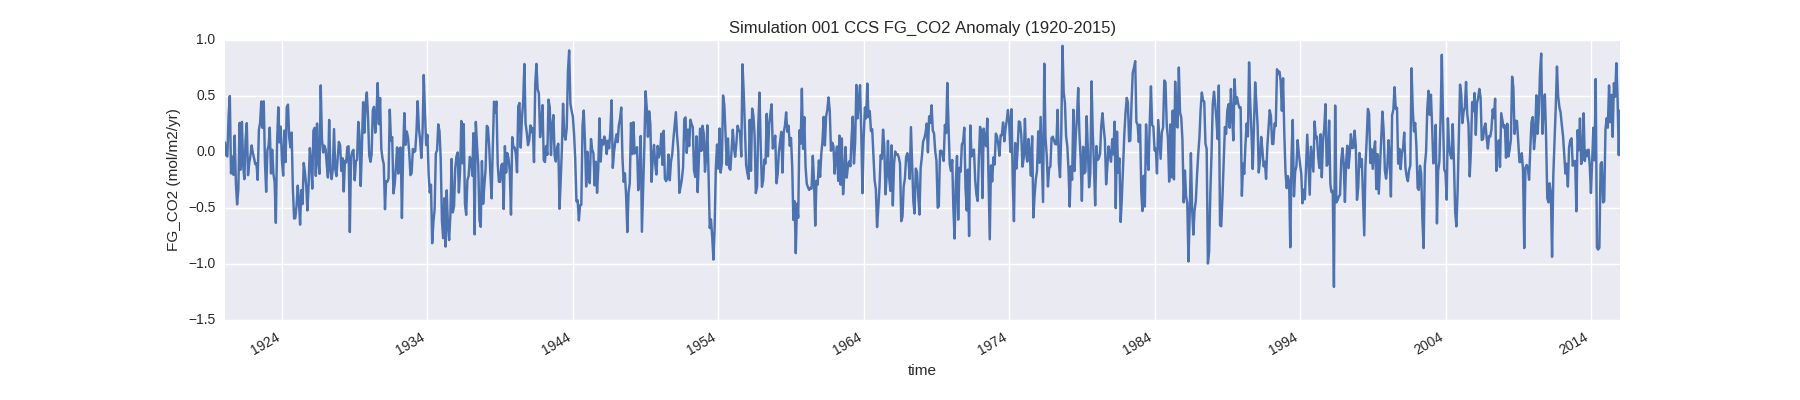
\includegraphics[width=\linewidth]{../../figs/CCS/timeseries/ccs-unfiltered-fgco2-series-example.png}
	\caption{Area-weighted average FGCO2 anomalies (ensemble mean removed) for simulation 001 over the domain in Figure~\ref{fig:1}.}
	\label{fig:2}
\end{figure}

We can apply a quick 12-month (annual) rolling mean to smooth out some of the noisiness. Figure~\ref{fig:3} shows the smoothed time series in black for simulation 001 (with the original unfiltered time series from Figure~\ref{fig:2} in blue). We only lose 11 data points on a 1140 length array by smoothing. 
\begin{figure}[!h]
	\centering
	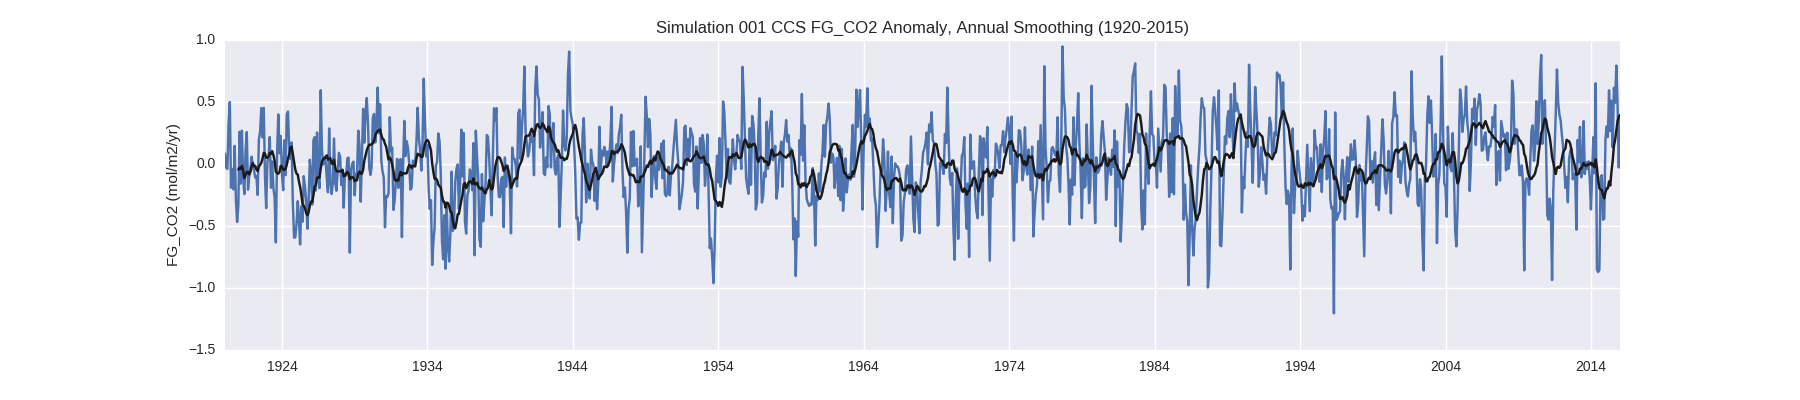
\includegraphics[width=\linewidth]{../../figs/CCS/timeseries/ccs-filtered-fgco2-series-example.png}
	\caption{Area-weighted average FGCO2 anomalies (ensemble mean removed) for simulation 001 over the domain in Figure~\ref{fig:1}.}
	\label{fig:3}
\end{figure}

An FFT of Figure~\ref{fig:2} is fairly inconclusive. At the very least, there is power at lower frequencies that diminishes at higher frequencies. It looks more red than white.
\newpage
\begin{figure}[!h]
	\centering
	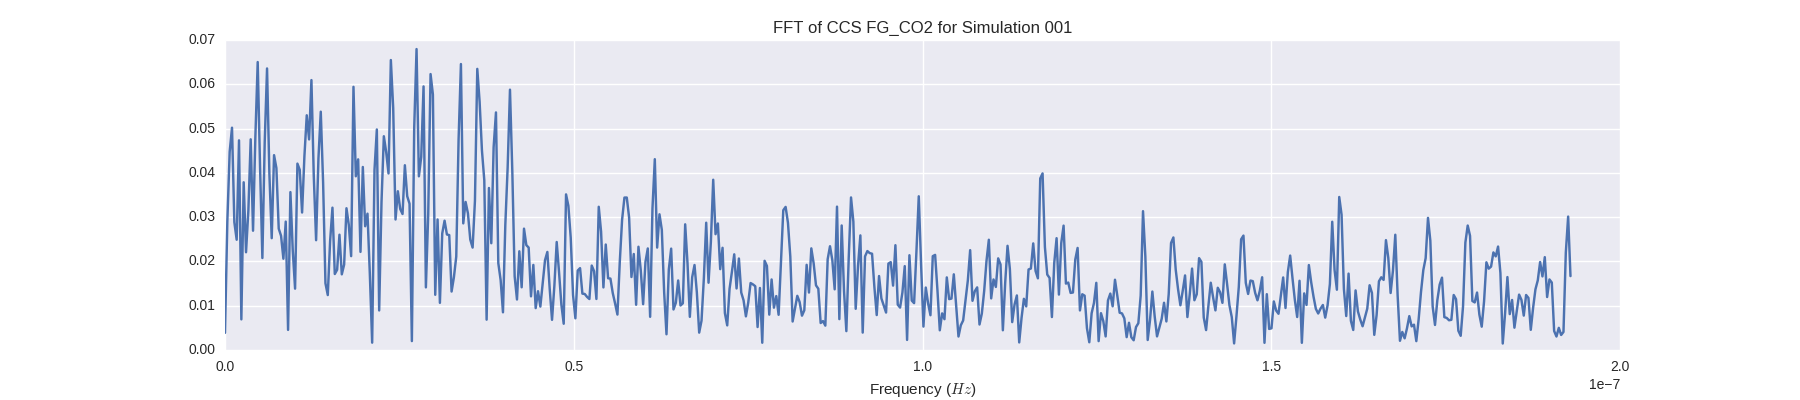
\includegraphics[width=\linewidth]{../../figs/CCS/fft/fft-CCS-001-frequencyHz.png}
	\caption{Area-weighted average FGCO2 anomalies (ensemble mean removed) for simulation 001 over the domain in Figure~\ref{fig:1}.}
	\label{fig:4}
\end{figure}

Now smoothed, the FGCO2 anomalies vary more closely with the Nino3.4 index, and even moreso with the PDO index.
\begin{figure}[!h]
	\centering
	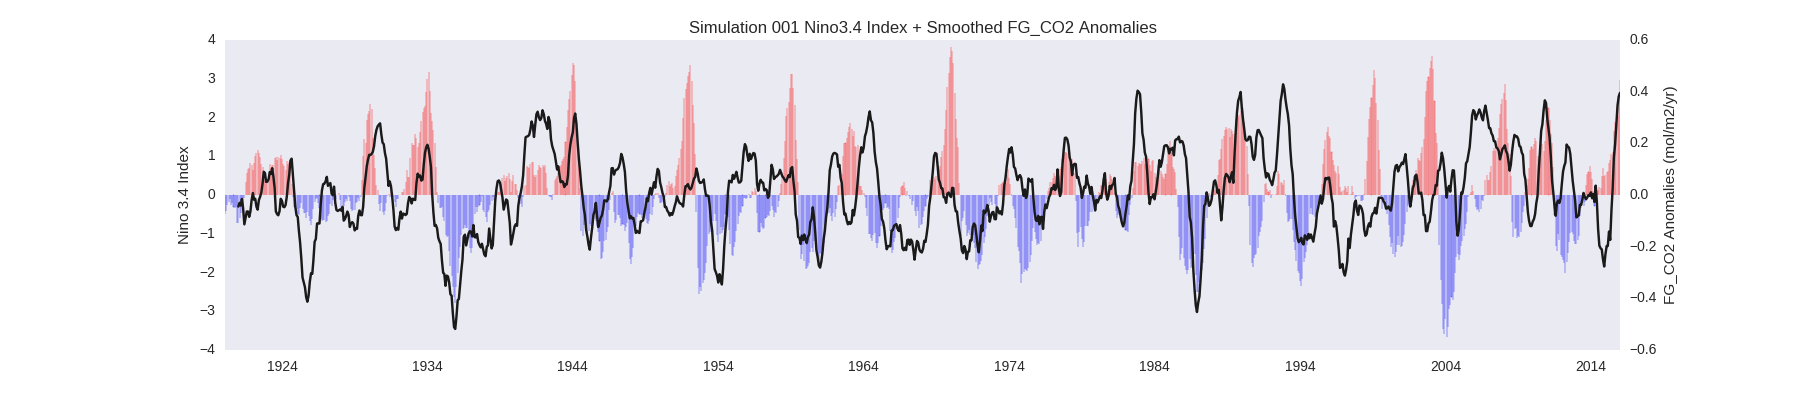
\includegraphics[width=\linewidth]{../../figs/CCS/timeseries/ccs-smoothed-fgco2-and-nino34-plot.png}
	\caption{Area-weighted average FGCO2 anomalies for simulation 001 with a one-year moving average applied (black line). The bar plot reflects the detrended Nino3.4 index from the same simulation.}
	\label{fig:5}
\end{figure}
\begin{figure}[!h]
	\centering
	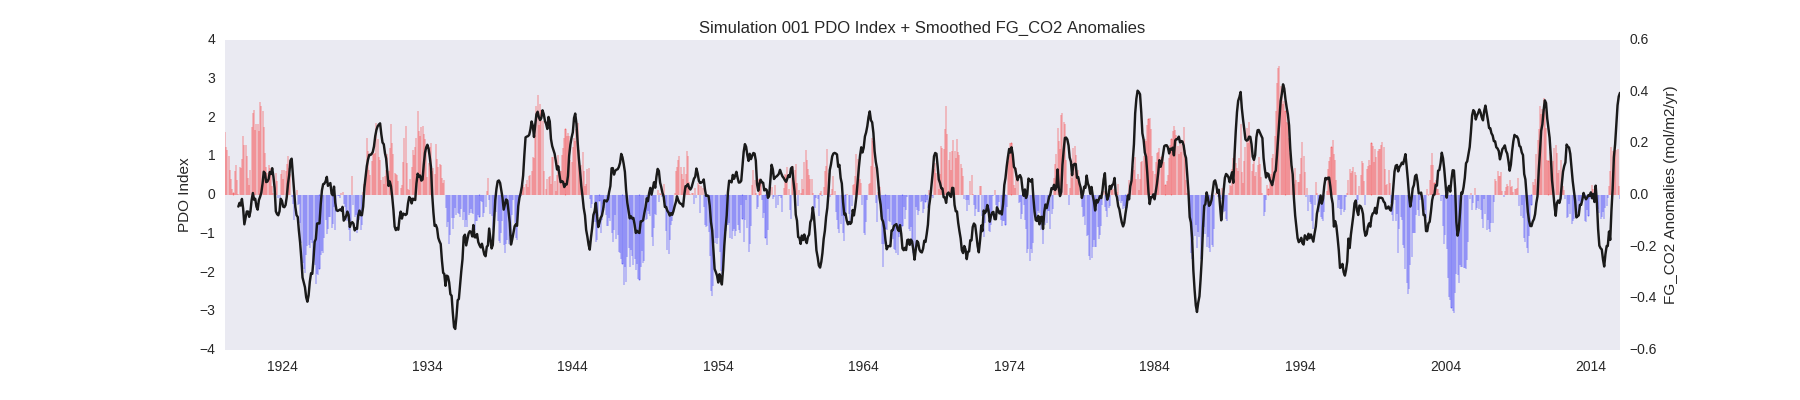
\includegraphics[width=\linewidth]{../../figs/CCS/timeseries/ccs-smoothed-fgco2-and-pdo-plot.png}
	\caption{Same as Figure~\ref{fig:5}, but with the PDO index.}
	\label{fig:6}
\end{figure}

\subsection{Regressing onto Climate Indices}
I can now regress these smoothed FGCO2 anomalies onto three main predictors: Nino3.4, PDO, and NPO (the last of which isn't covered here due to low correlation values). Figure~\ref{fig:7} displays a scatter plot for all 34 ensemble members comparing their r-value for ENSO to their r-value for PDO. Save for one outlier in the bottom left, simulations cluster generally toward strong correlations for both metrics, favoring the PDO index. Table~\ref{tab:1} and Table~\ref{tab:2} display raw results (R value, R$^{2}$, and regression coefficient) for every simulation.
\newpage
\begin{figure}[!h]
	\centering
	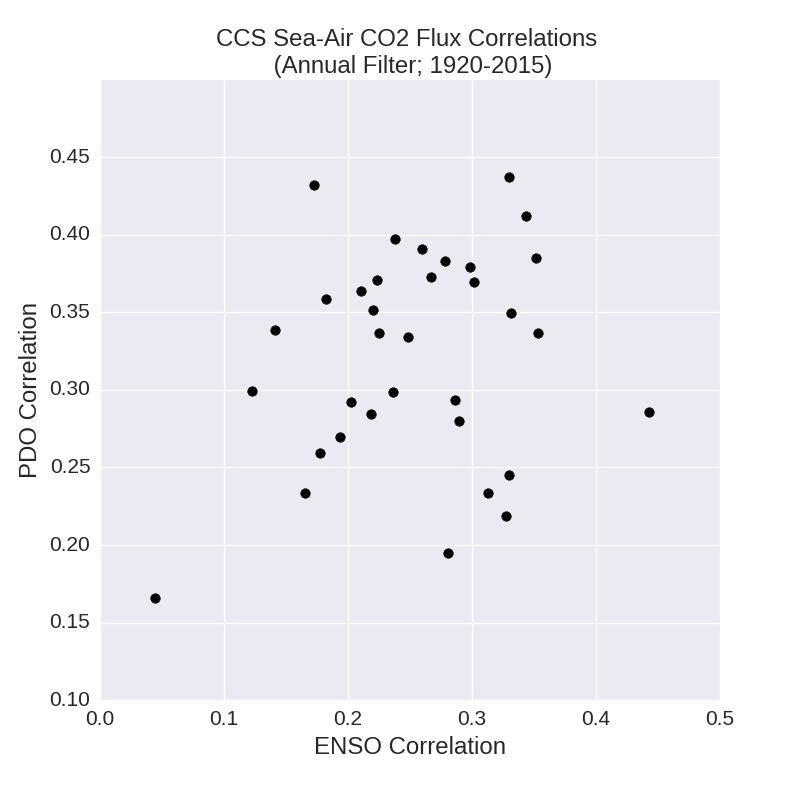
\includegraphics[width=25pc]{../../figs/CCS/correlations_scatter/CCS-ENSO-PDO-Correlation-Scatter.png}
	\caption{R values for annually smoothed FGCO2 anomalies in the CCS compared to Nino3.4 and PDO indices for all 34 ensemble members.}
	\label{fig:7}
\end{figure}
\begin{figure}[!h]
	\centering
	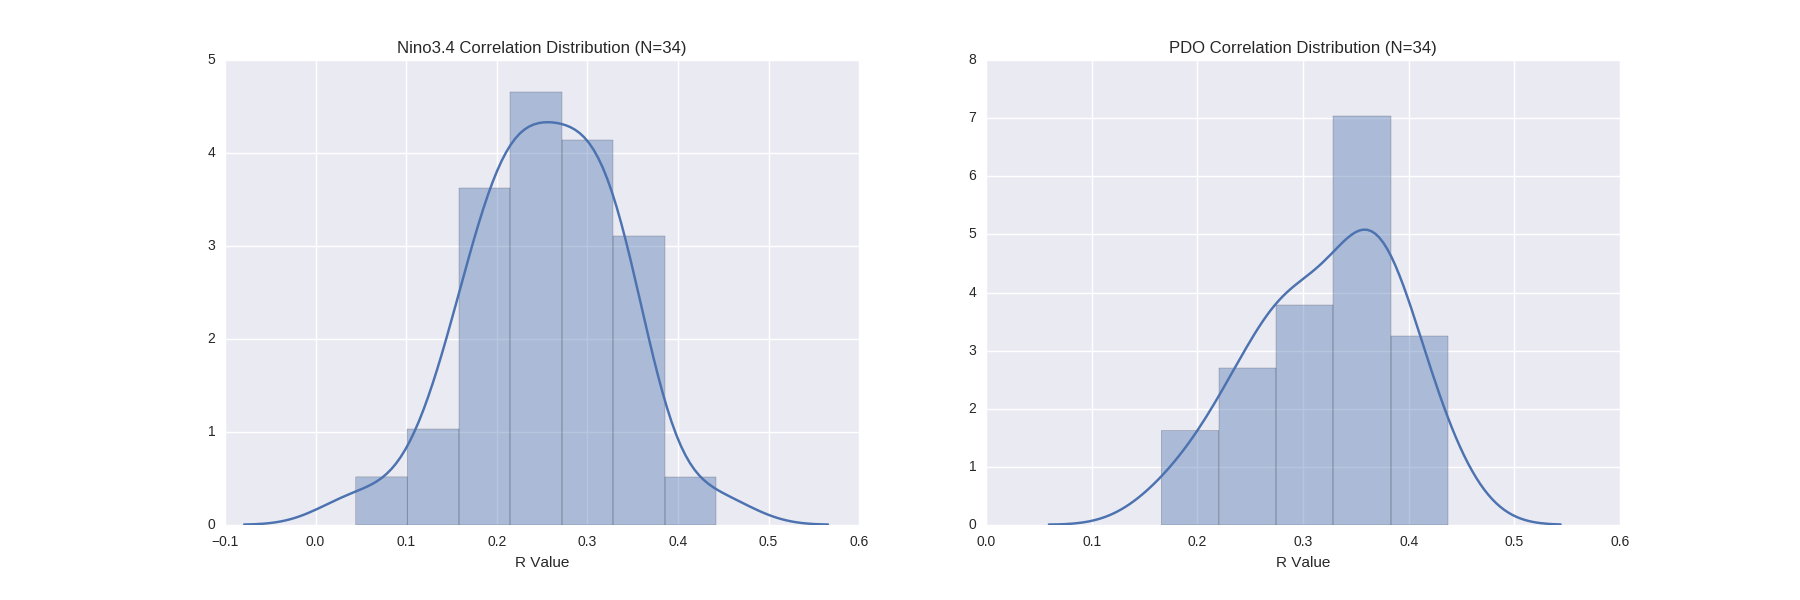
\includegraphics[width=39pc]{../../figs/CCS/correlations_scatter/ensemble-correlation-distribution-enso+pdo.png}
	\caption{Distribution of correlations between smoothed FGCO2 anomalies and Nino3.4/PDO indices.}
	\label{fig:8}
\end{figure}

\newpage
\begin{table}[!h]
\centering
\caption{Regression Results by simulation, with Nino3.4 index as the predictor and FGCO2 anomalies as the criterion. All results have a p-value $<<$ 0.05.}
\begin{tabular}{c | c c c}
	\toprule
	\textbf{Simulation} &  \textbf{Slope} [mol/m$^{2}$/yr/degC] &  \textbf{R} &  \textbf{R$^{2}$} \\
	\midrule
	001 &   0.04 &     0.30 &       0.09 \\
	002 &   0.06 &     0.33 &       0.11 \\
	009 &   0.03 &     0.18 &       0.03 \\
	010 &   0.04 &     0.22 &       0.05 \\
	011 &   0.01 &     0.04 &       0.00 \\
	012 &   0.05 &     0.28 &       0.08 \\
	013 &   0.06 &     0.33 &       0.11 \\
	014 &   0.05 &     0.35 &       0.12 \\
	015 &   0.05 &     0.29 &       0.08 \\
	016 &   0.04 &     0.22 &       0.05 \\
	017 &   0.04 &     0.27 &       0.07 \\
	018 &   0.05 &     0.29 &       0.08 \\
	019 &   0.04 &     0.21 &       0.04 \\
	020 &   0.05 &     0.30 &       0.09 \\
	021 &   0.03 &     0.18 &       0.03 \\
	022 &   0.04 &     0.24 &       0.06 \\
	023 &   0.03 &     0.22 &       0.05 \\
	024 &   0.06 &     0.33 &       0.11 \\
	025 &   0.05 &     0.34 &       0.12 \\
	026 &   0.04 &     0.25 &       0.06 \\
	027 &   0.04 &     0.28 &       0.08 \\
	028 &   0.03 &     0.17 &       0.03 \\
	029 &   0.05 &     0.33 &       0.11 \\
	030 &   0.03 &     0.19 &       0.04 \\
	031 &   0.04 &     0.24 &       0.06 \\
	032 &   0.04 &     0.20 &       0.04 \\
	033 &   0.02 &     0.14 &       0.02 \\
	034 &   0.06 &     0.31 &       0.10 \\
	035 &   0.03 &     0.17 &       0.03 \\
	101 &   0.07 &     0.44 &       0.20 \\
	102 &   0.04 &     0.26 &       0.07 \\
	103 &   0.04 &     0.22 &       0.05 \\
	104 &   0.05 &     0.35 &       0.12 \\
	105 &   0.02 &     0.12 &       0.01 \\
	\bottomrule
	\textbf{Mean} & 0.04 & 0.25 & 0.07 \\
	\textbf{Std. Dev} & 0.01 & 0.08 & 0.04 \\
\end{tabular}
\label{tab:1}
\end{table}
\newpage
\begin{table}[!h]
\centering
\caption{Same as Table~\ref{tab:1}, but as compared to the PDO index}
\begin{tabular}{c | c c c}
	\toprule
	\textbf{Simulation} &  \textbf{Slope} [mol/m$^{2}$/yr/degC] &  \textbf{R} &  \textbf{R$^{2}$} \\
	\midrule
	001 &   0.06 &     0.38 &       0.14 \\
	002 &   0.06 &     0.35 &       0.12 \\
	009 &   0.06 &     0.36 &       0.13 \\
	010 &   0.06 &     0.35 &       0.12 \\
	011 &   0.03 &     0.17 &       0.03 \\
	012 &   0.07 &     0.38 &       0.15 \\
	013 &   0.04 &     0.25 &       0.06 \\
	014 &   0.06 &     0.34 &       0.11 \\
	015 &   0.05 &     0.29 &       0.09 \\
	016 &   0.05 &     0.28 &       0.08 \\
	017 &   0.06 &     0.37 &       0.14 \\
	018 &   0.05 &     0.28 &       0.08 \\
	019 &   0.07 &     0.36 &       0.13 \\
	020 &   0.06 &     0.37 &       0.14 \\
	021 &   0.04 &     0.26 &       0.07 \\
	022 &   0.07 &     0.40 &       0.16 \\
	023 &   0.05 &     0.37 &       0.14 \\
	024 &   0.08 &     0.44 &       0.19 \\
	025 &   0.07 &     0.41 &       0.17 \\
	026 &   0.05 &     0.33 &       0.11 \\
	027 &   0.03 &     0.19 &       0.04 \\
	028 &   0.07 &     0.43 &       0.19 \\
	029 &   0.03 &     0.22 &       0.05 \\
	030 &   0.05 &     0.27 &       0.07 \\
	031 &   0.05 &     0.30 &       0.09 \\
	032 &   0.05 &     0.29 &       0.09 \\
	033 &   0.05 &     0.34 &       0.11 \\
	034 &   0.04 &     0.23 &       0.05 \\
	035 &   0.04 &     0.23 &       0.05 \\
	101 &   0.05 &     0.29 &       0.08 \\
	102 &   0.07 &     0.39 &       0.15 \\
	103 &   0.06 &     0.34 &       0.11 \\
	104 &   0.06 &     0.39 &       0.15 \\
	105 &   0.05 &     0.30 &       0.09 \\
	\bottomrule
	\textbf{Mean} & 0.05 & 0.32 & 0.11 \\
	\textbf{Std. Dev} & 0.01 & 0.07 & 0.04 \\
\end{tabular}
\label{tab:2}
\end{table}

\bibliography{../../EBUS_BGC_Bibliography.bib}
\end{document}
